%----------------------------------------------------------------------------------------
%	PACKAGES AND OTHER DOCUMENT CONFIGURATIONS
%----------------------------------------------------------------------------------------

\documentclass[paper=a4, fontsize=11pt]{scrartcl} % A4 paper and 11pt font size

% ---- Entrada y salida de texto -----

\usepackage[T1]{fontenc} % Use 8-bit encoding that has 256 glyphs
\usepackage[utf8]{inputenc}
%\usepackage{fourier} % Use the Adobe Utopia font for the document - comment this line to return to the LaTeX default

% ---- Idioma --------

\usepackage[spanish, es-tabla]{babel} % Selecciona el español para palabras introducidas automáticamente, p.ej. "septiembre" en la fecha y especifica que se use la palabra Tabla en vez de Cuadro

% ---- Otros paquetes ----
\usepackage{csquotes} %Para permitir el uso de comillas Quotes https://tex.stackexchange.com/questions/36812/isnt-there-any-other-way-of-doing-double-quotes-in-latex-besides
\usepackage[hyphens]{url} % ,href} %para incluir URLs e hipervínculos dentro del texto (aunque hay que instalar href)
\usepackage{hyperref}
\usepackage{color}
\usepackage{graphics,graphicx, floatrow} %para incluir imágenes y notas en las imágenes
\usepackage{graphics,graphicx, float} %para incluir imágenes y colocarlas

\graphicspath {{./img/}}

\usepackage{listings}  %para introducir comandos

\lstdefinestyle{mybash}
{basicstyle=\ttfamily,
  showstringspaces=false,
  commentstyle=\color{red},
  keywordstyle=\color{blue},
  language=bash,
  alsoletter=/,
  basicstyle=\footnotesize,
  numbers=left,
  stepnumber=1,
  showstringspaces=false,
  tabsize=1,
  breaklines=true,
  breakatwhitespace=false,
}
\lstdefinestyle{mysql}
{basicstyle=\ttfamily,
  showstringspaces=false,
  commentstyle=\color{red},
  keywordstyle=\color{blue},
  language=sql,
  basicstyle=\footnotesize,
  numbers=left,
  stepnumber=1,
  showstringspaces=false,
  tabsize=1,
  breaklines=true,
  breakatwhitespace=false,
}


% Para hacer tablas comlejas
%\usepackage{multirow}
%\usepackage{threeparttable}

%\usepackage{sectsty} % Allows customizing section commands
%\allsectionsfont{\centering \normalfont\scshape} % Make all sections centered, the default font and small caps

\usepackage{fancyhdr} % Custom headers and footers
\pagestyle{fancyplain} % Makes all pages in the document conform to the custom headers and footers
\fancyhead{} % No page header - if you want one, create it in the same way as the footers below
\fancyfoot[L]{} % Empty left footer
\fancyfoot[C]{} % Empty center footer
\fancyfoot[R]{\thepage} % Page numbering for right footer
\renewcommand{\headrulewidth}{0pt} % Remove header underlines
\renewcommand{\footrulewidth}{0pt} % Remove footer underlines
\setlength{\headheight}{13.6pt} % Customize the height of the header

\setlength\parindent{0pt} % Removes all indentation from paragraphs - comment this line for an assignment with lots of text

\newcommand{\horrule}[1]{\rule{\linewidth}{#1}} % Create horizontal rule command with 1 argument of height


%----------------------------------------------------------------------------------------
%	TÍTULO Y DATOS DEL ALUMNO
%----------------------------------------------------------------------------------------
\graphicspath{ {img/} }

\title{
\normalfont \normalsize

\includegraphics[width=6cm,height=6cm]{logo}\\
\textsc{\textbf{Bootcamp Especialidad GNU/Linux (2023)}} \\ [25pt] % Your university, school and/or department name(s)
\horrule{0.5pt} \\[0.4cm] % Thin top horizontal rule
\huge Lab 06 - NFS \\ % The assignment title
\horrule{2pt} \\[0.5cm] % Thick bottom horizontal rule
}


%https://es.overleaf.com/learn/latex/Inserting_Images
%Ruta relativa de   imagenes

\author{Pedro Antonio Mayorgas Parejo} % Nombre y apellidos

\date{\normalsize\today} % Incluye la fecha actual

%----------------------------------------------------------------------------------------
% DOCUMENTO
%----------------------------------------------------------------------------------------

\begin{document}

\maketitle % Muestra el Título

\newpage %inserta un salto de página

\tableofcontents % para generar el índice de contenidos

\newpage

%----------------------------------------------------------------------------------------
%	Cuestión 1
%----------------------------------------------------------------------------------------

\section{Instalación de NFS Server}

% \vspace{5mm}

Para la instalación de NFS, necesitamos el siguiente paquete:

\begin{lstlisting}[style=mybash]
sudo apt install nfs-kernel-server
\end{lstlisting}

\begin{figure}[H]
	\centering
	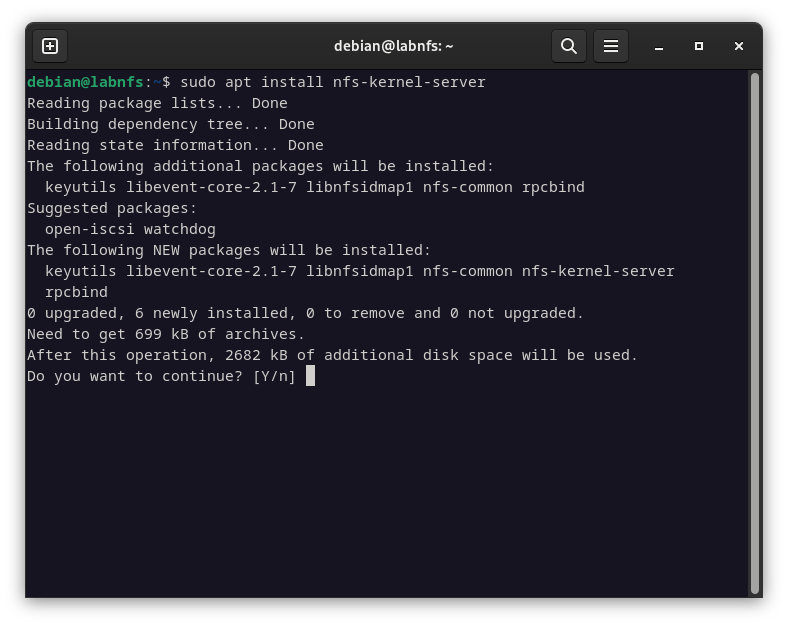
\includegraphics[scale=0.30]{00}
	\caption{Instalación del servicio NFS.}
\end{figure}


Ahora creamos una carpeta en /srv/data, para que esté lista para la exportación de NFS. Le cambiamos el usuario y grupo, de manera que permitamos que los usuarios ajenos puedan escribir/leer/ejecutar en ellas. Esto debe ser combinado con el all\_squash (si queremos que todos los usuarios no tengan permisos especiales), o root\_squash (si queremos que el usuario root no tenga permisos de superusuario).

\begin{lstlisting}[style=mybash]
sudo mkdir /srv/data
sudo chown -R nobody:nogroup /srv/data
\end{lstlisting}

Luego a continuación vamos al fichero localizado en \textbf{/etc/exports}, donde en ese fichero indicamos la exportación de la carpeta.

\begin{lstlisting}[style=mybash]
sudo nano /etc/exports
# Dentro del fichero
/srv/data 192.168.122.0/24(rw,no_subtree_check,sync,all_squash)
# Luego, activamos y comprobamos el servicio
systemctl enable nfs-kernel-server
sudo systemctl start nfs-kernel-server
sudo systemctl status nfs-kernel-server
# Exportamos el directorio
sudo exportfs -ra
# Verificamos el export
sudo exportfs
\end{lstlisting}

\begin{figure}[H]
	\centering
	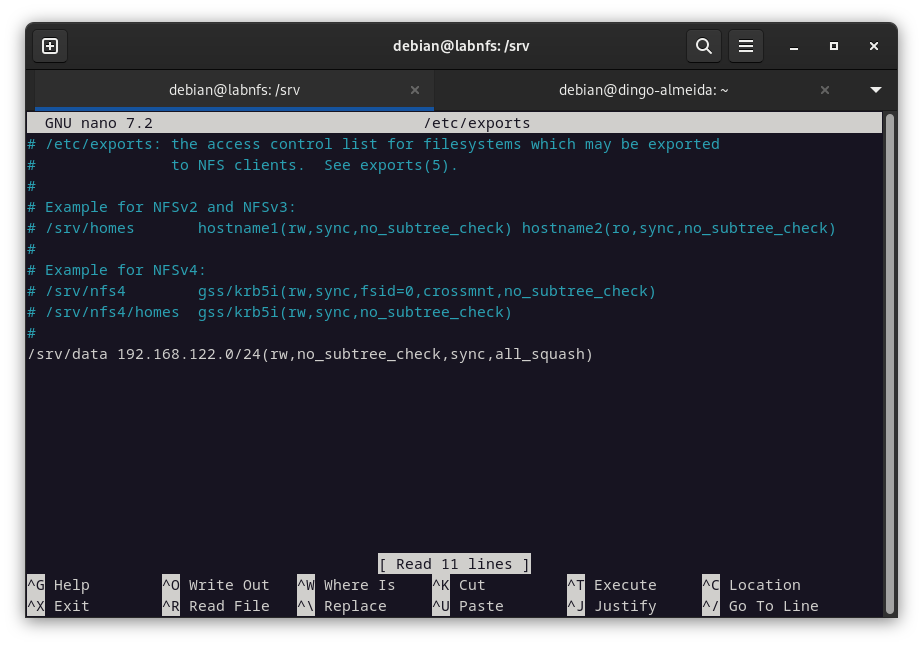
\includegraphics[scale=0.30]{01}
	\caption{Fichero /etc/exports.}
\end{figure}

\begin{enumerate}
\item 192.168.122.0/24 - Indicamos la subred permitida.
\item rw - Permitimos la escritura y lectura.
\item sync - Modo de sincronización total, indica al servidor NFS que expere a terminar una petición antes de atender la siguiente.
\item all\_squash - Indica que todos los usuarios serán identificados como nobody.
\item no\_subtree\_check - Indicamos al sistema NFS, que no tenga en cuenta los permisos root en el sistema de ficheros original, es decir dentro de los subdirectorios exportados.
\end{enumerate}

\begin{figure}[H]
	\centering
	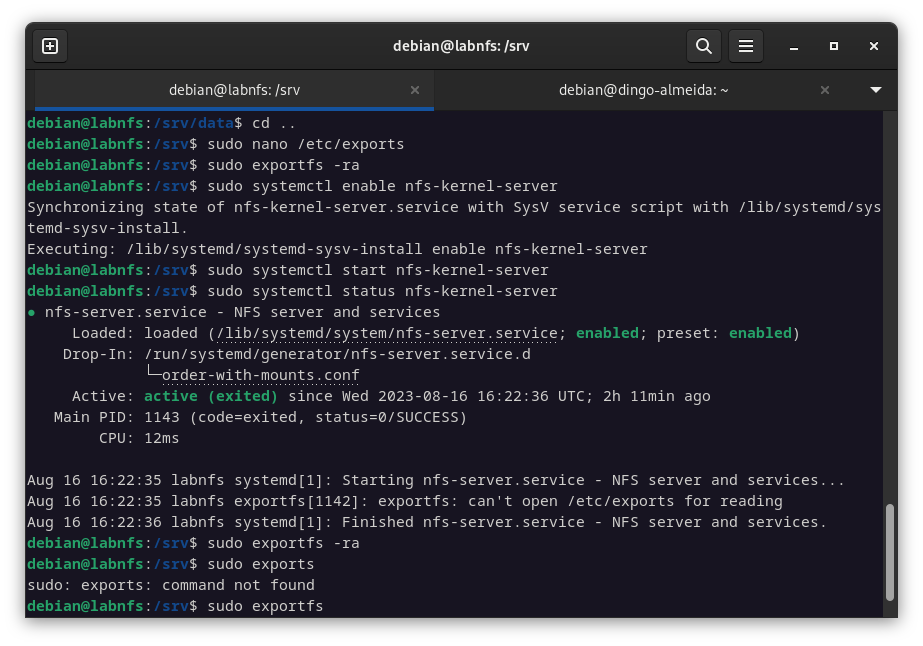
\includegraphics[scale=0.30]{02}
	\caption{Activación del servicio y exportación del directorio.}
\end{figure}

\newpage
\section{Cliente NFS}

Para el cliente instalamos el siguiente paquete:

\begin{lstlisting}[style=mybash]
sudo apt install nfs-common
\end{lstlisting}

\begin{figure}[H]
	\centering
	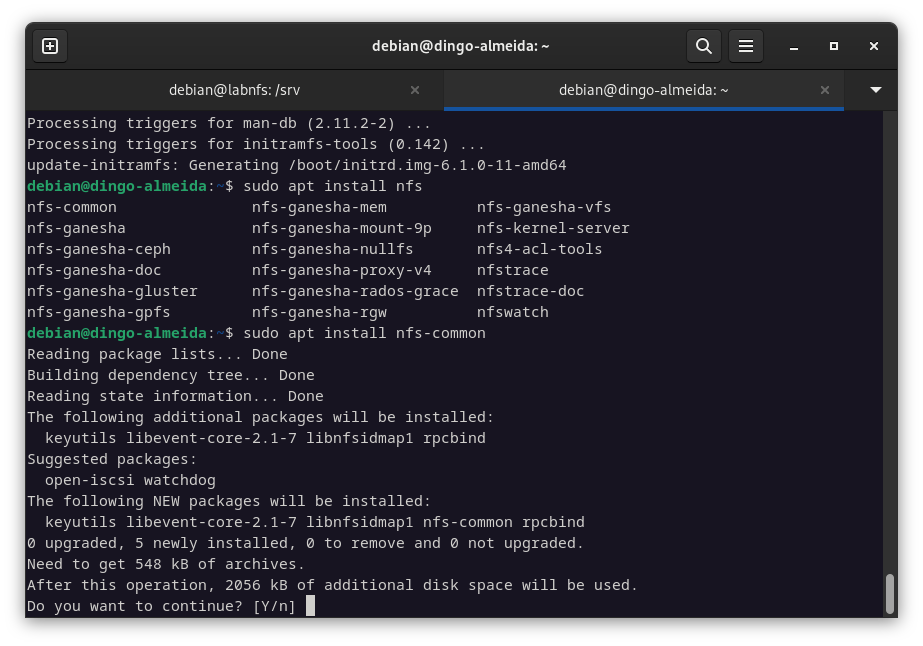
\includegraphics[scale=0.30]{03}
	\caption{Instalación del paquete.}
\end{figure}

Después de instalarlo, comprobamos la disponibilidad de los puntos de exportación, lo montamos con mount para hacer la prueba y finalmente creamos los ficheros o directorios dentro de ella para poder probar el sistema NFS.
\begin{lstlisting}[style=mybash]
# Buscamos el servidor NFS
sudo showmount -e 192.168.122.4
# Creamos la carpeta de montaje
sudo mkdir -p /var/www/html/DATA
# Montamos manualmente
sudo mount -t nfs4 192.168.122.4:/srv/data /var/www/html/DATA
\end{lstlisting}

\begin{figure}[H]
	\centering
	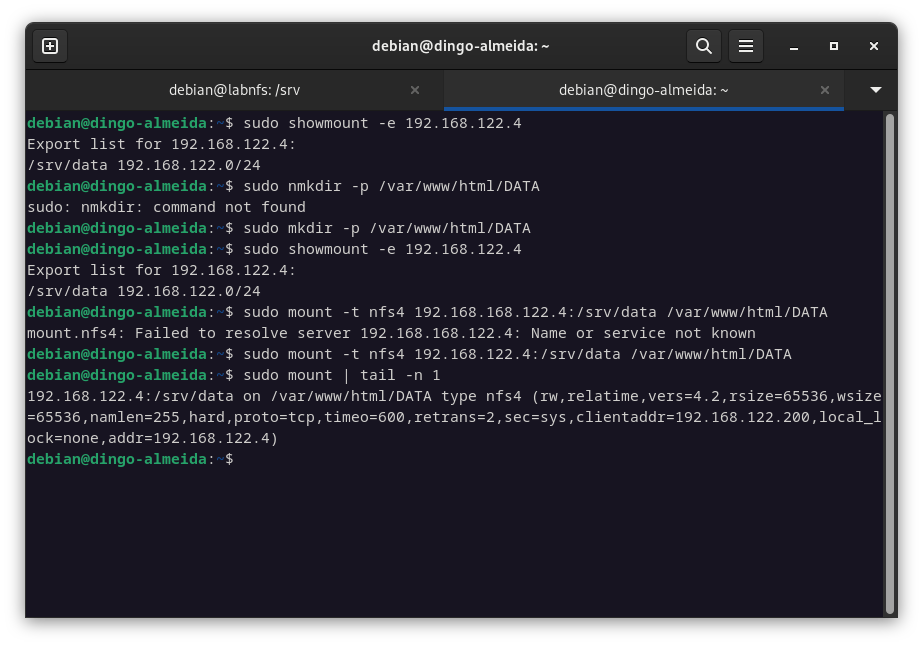
\includegraphics[scale=0.30]{04}
	\caption{Comprobando disponibilidad y montaje manual.}
\end{figure}

\begin{figure}[H]
	\centering
	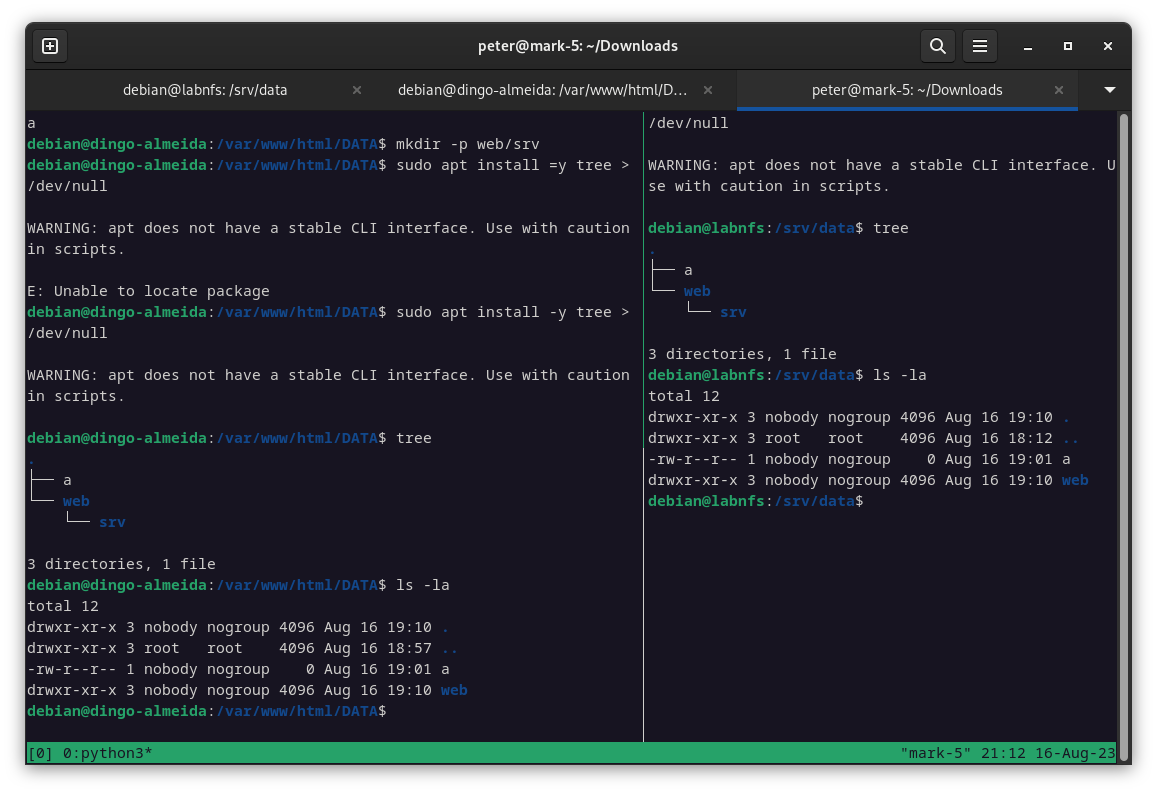
\includegraphics[scale=0.30]{05}
	\caption{Pruebas de creación de directorios.}
\end{figure}

\subsection{Persistencia de NFS en el cliente}

Para que el cliente cada vez que arranque su sistema pueda montar la exportación de manera automática. Tenemos que crear la siguiente entrada en \textbf{/etc/fstab}.
\begin{lstlisting}[style=mybash]
# NFS EXPORT
192.168.122.4:/srv/data /var/www/html/DATA nfs4 defaults,rw	0	0
\end{lstlisting}

\begin{figure}[H]
	\centering
	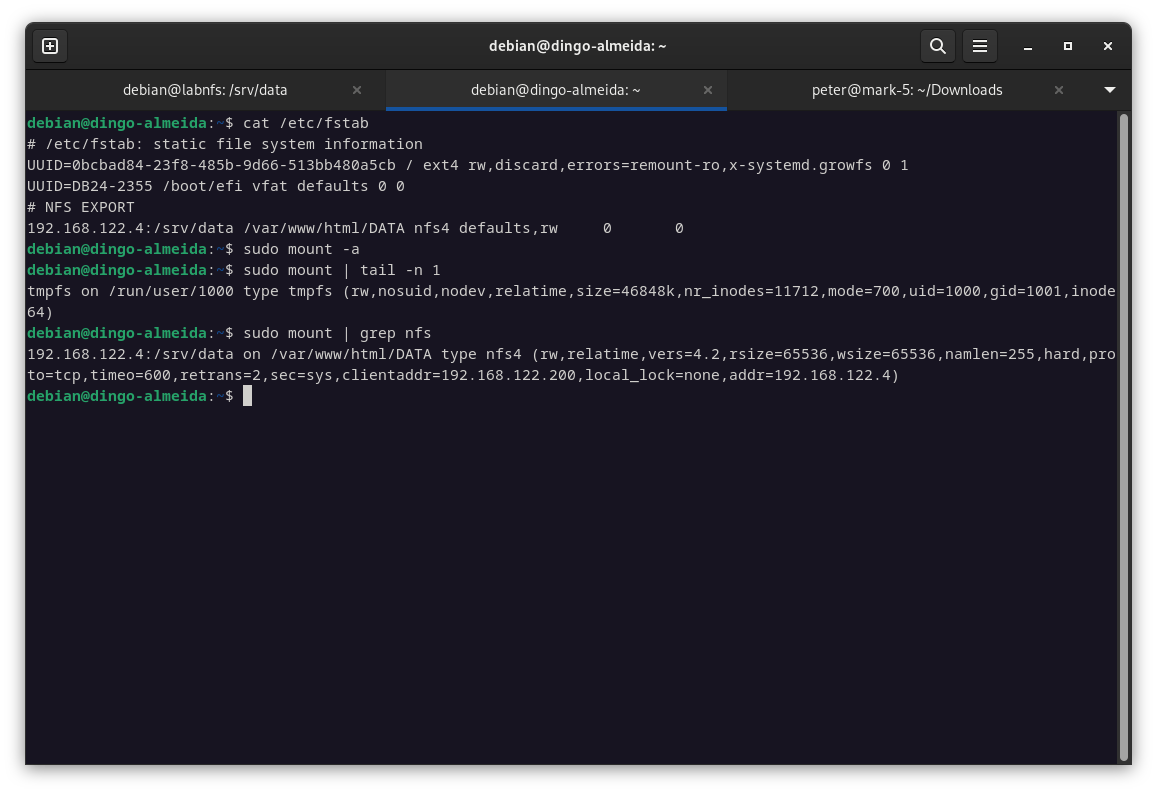
\includegraphics[scale=0.30]{06}
	\caption{Montaje automático.}
\end{figure}
% \begin{lstlisting}[style=mybash]
%     # Para una base de datos concreta
%     mysqldump --user=tiendabd --password=password --databases tiendabd --add-drop-database --add-drop-table [--replace] --host=127.0.0.1 --result-file=dump.sql
% \end{lstlisting}



%\begin{figure}[H]
%	\centering
%	\includegraphics[scale=0.30]{cuestion\_1\_1}
%	\caption{Se puede ver que al no haber un fallo grave, el sistema lo nota como que sigue funcionando pero en un estado degradado.}
%\end{figure}

%\newpage

%Se pueden hacer include en latex
%\input{plantilla\_include.tex}


%-------Bibliografia-----------------------------

%\newpage
\section{Bibliografía}

% Ejemplo
\footnote{Administración de mdadm - Por Red Hat}
\textcolor{blue}{\url{https://access.redhat.com/documentation/en-us/red_hat_enterprise_linux/8/html/managing_storage_devices/managing-raid_managing-storage-devices#monitoring-raid_managing-raid}}



\end{document}
